\documentclass[12pt,a4paper]{book}
\usepackage[utf8]{inputenc}
\usepackage[hangul]{kotex}
\usepackage{amsmath}
\usepackage{amsfonts}
\usepackage{amssymb}
\usepackage{graphicx}
\usepackage{graphicx,subcaption}
\usepackage[left=2cm,right=2cm,top=2cm,bottom=2cm]{geometry}
\author{강명세}
\title{사회적 선호는 정치적으로 얼마나 반영돼는가?}
\begin{document}
민주주의는  얼마나 시민 다수가 희망하는 반영하는가? 이 질문은 당연한 듯하지만 현실은 그렇지 않다. 역사적으로 민주주의는 다수의 선호를 반영하는 방향으로 움직였으나 제도적 매개에 따라 선호의 반영에는 여전히 많은 차이가 존재한다 국가별로도 중대한 차이가 있다. 어떤 곳에서는 공공영역이 크게 팽창한 반면 미국처럼 "작은 정부의 미덕"이 뿌리내린 곳도 있다. 
민주주의에서 사회정책은 중요하다. 의료보험, 실업연금 및 노후연금 등을 포괄하는 사회정책은 소득분포에 영향을 주는 점에서 시민은 그 향배에 큰 관심을 갖는다. 개개인은 스스로에게 귀속하는 다양한 속성에 따라  사회적 선호를 형성한다. 자신의 이익을 극대화하면서 사회적 형평성에도 관심을 갖는다. 사회적 선호가 얼마나 반영되는가는 민주주의가 얼마나 민주적인가를 반영하는 것이다.  사회적 선호와 민주주의의 관계에 대해서는 많은 논의가 있어 왔다. 중위투표자 가설은 중위투표자가 조세와 재분배의 폭을 결정한다고 주장했다.\footnote{중위가설을 대중화시킨 것은 Meltzer and Ricard 1981}\footnote{ 이들의 논문 제목 \textit{The Size of Government}자체가 말해준다} 민주주의의 불평등성을 지적하는 논의가 있다. 한편 최근  민주주의에서 정당과 정부는 다수의 이해와 이익을 위한 정책을 개방하고 실시한다는 주장이 제시된 바 있다.\footnote{Brooks and Manza 2006; Soroka \& Wlezien 2005} 중위가설은 경험적으로 애매한 검증을 받아왔다. 부분적으로 부합하는 연구가 있는 반면 가설을 부정하는 결과도 제시되었다. 

한편 민주적 대응의 전통에 대해 정책편견에 대한 우려가 도전한다. 미국에서 발생한 대침체(Great Recession)가 지속되면서 민주주의의 불평등성이 제기되면서 미국 민주주의의 위기를 경고하였다. 경제적 불평등은 민주주의를 지탱하는 \textit{일인 일표}의 제어를 받지 않고 정치적 불평등으로 발전한다는 것이다. 이들은 선거에서 갈수록 정치자금이 결정한다는 점에 주목한다. 경제적 힘은 선거에서 미디어를 통해 부유층을 대변하는 후보와 정당을 지지한다는 점을 경험적으로 증명하려고 노력한다. \footnote{Gilens(2005)의 연구와 Bartels(2008)는 이 분야의 선두 주자이며 많은 후속연구가 진행 중에 있다:  Gilens(2012) Bartels(2017); Gilens \& Page(2014)} 이들의 연구는 다수의 사회적 선호가 아니라 소수의 선호가 반영된다는 점을 강조한다. 비판이론은 정부가 저소득자나 중간층의 의견을 무시하고 부유층의 입장을 반영한다는 점을 주장한다. 저소득  홀대론은 최근 확산 일로에 있다.  홀대론은 전통적 이론의 관점은 누구의 이해가 반영되는지에 대해서가 아니라 어떻게 반영되는가를 초점을 두며 따라서 초점이 다르다고 주장한다(Bartels 2017, 6).

정부의 규모에 대한 또 다른 이론은 \textit{권력자원이론,power resouce theory}은이다. 그것은 중위투표자 이론과는 달리  사회집단이나 계급이 보유한 자원에 따라 정부정책의 성격이 결정된다고 본다. 권력자원론은 왜 국가별로 정부규모가 서로 다른가에 주목했다. 스웨덴같이 복지국가가 발전한 반면, 한국이나 미국처럼 복지가 저개발된 까닭은 무엇인가? 좌파의 세력이 강력하게 발전한 나라에서는 정부와 공공영역이 확대되었다는 결과를 제시했다.\footnote{개척적 연구는 John D. Stephens 1978 이후 중대한 흐름을 형성하고 후속연구에 막대한 영향을 미쳤다; Esping-Andersen1990; ;Huber \& Stephens 2001} Huber \& Stepens는 사회주의 정당이 집권했던 경험은 사회정책의 강도에 지속적 영향을 준다는 점을 강조한다. 

\begin{figure}
\centering
        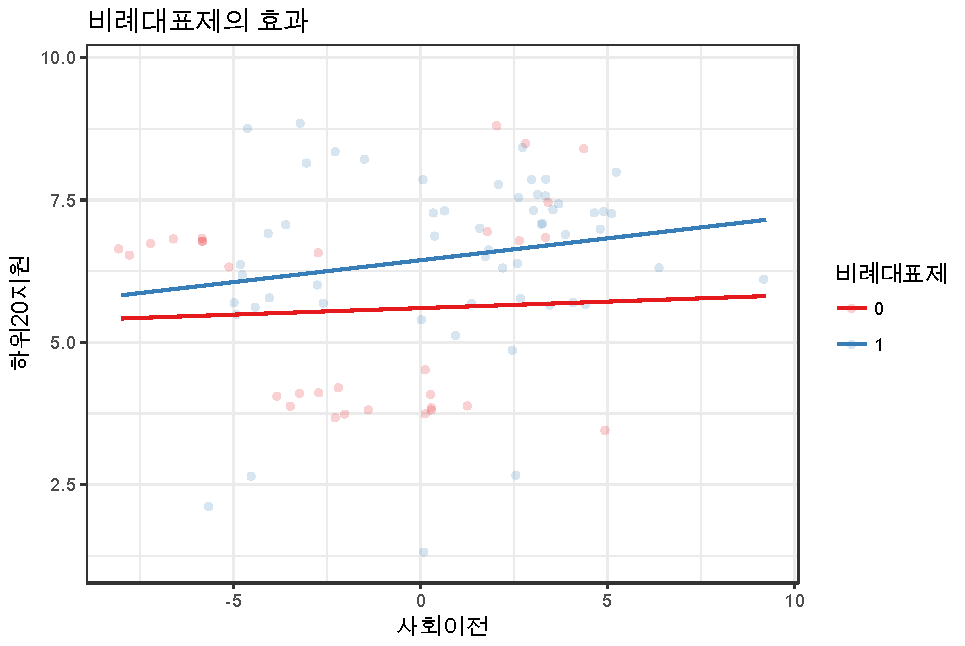
\includegraphics[width=0.9\textwidth]{pr_sstran.pdf}\\
        \caption{한국}
\end{figure}

비례대표제가 단순다수제에 비해 소수당의 집입이 용이하며 따라서 이 제도엣 저소득층의 이익을 대표하는 정당이 정책에 참여할 가능성이 높다.  저소득층을 지원하는 사회이전이 증가해도 다수제 민주주의에서는 하위20\%이 차지하는 비중은 변동이 없다. 그러나, 그림 1에서 보듯 비례대표제 민주주의에서는 사회이전지출이 증가할수록 하위20\%의 몫은 늘어난다. 저소득층의 지원에 영향을 주는 요인으로 사회지출, 좌파정당의 집권경험, 정부의 이념적 구성, 그리고 선거제도(비례대표제) 등으로 가정한 모형에서 사회이전은 최저 또는 최대로 하고 모든 변수 값은 중위값으로 책정한 뒤 저소득의 비중이 얼마나 증가하는 가를 비교해보면 5.87\%에서 6.85\%로 증가한다. 다시 말해, 다수제에서 보다 비례대표제 민주주의에서 재분배가 더 잘 작동하는 것이다. 비례대표제의 효과를 정확히 포착하기 위해서는 혼합모형(Mixed Model)을 적용해야 한다. 일반선형모델(glm)에서는 위계적 자료나 종단면 자료의 특성을 반영할 수 없다. 일반화선형모델(GLM)을 적용하면 비례대표제 요인은 통계적 유의성이 없다.\footnote{비례대표제의 회귀계수는 0.497이며 표준오차는 0.371으로 통계적 유의미하지 않다. 보다 상세한 논의는 Fox(2016) IV. The Mixed Effects Model 참고} \\

\begin{figure}
\centering
        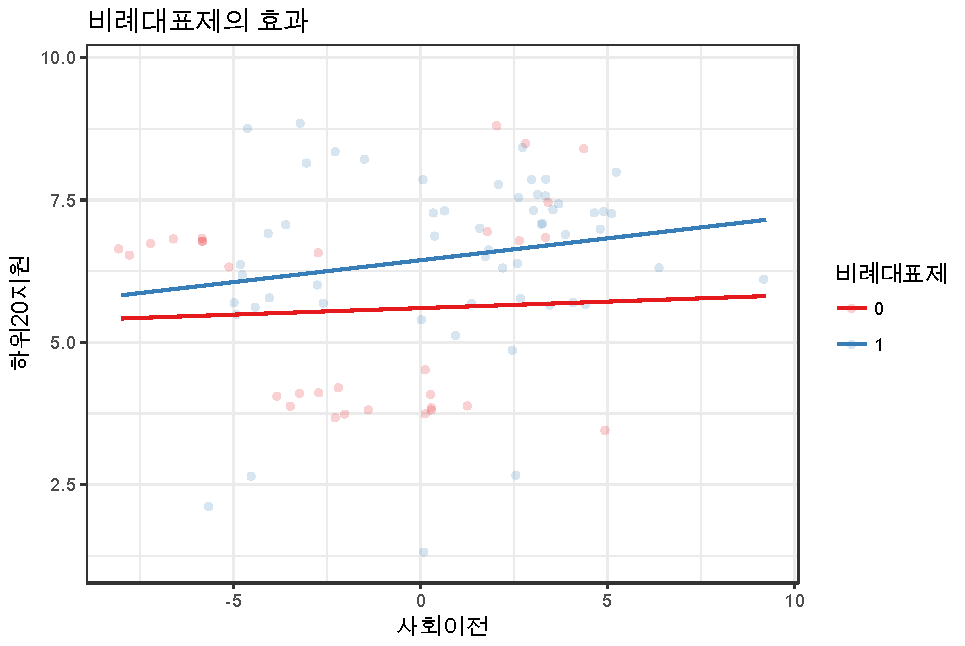
\includegraphics[width=0.9\textwidth]{pr_sstran.pdf}\\
        \caption{사회이전지출}
\end{figure}

\begin{figure}
\centering
        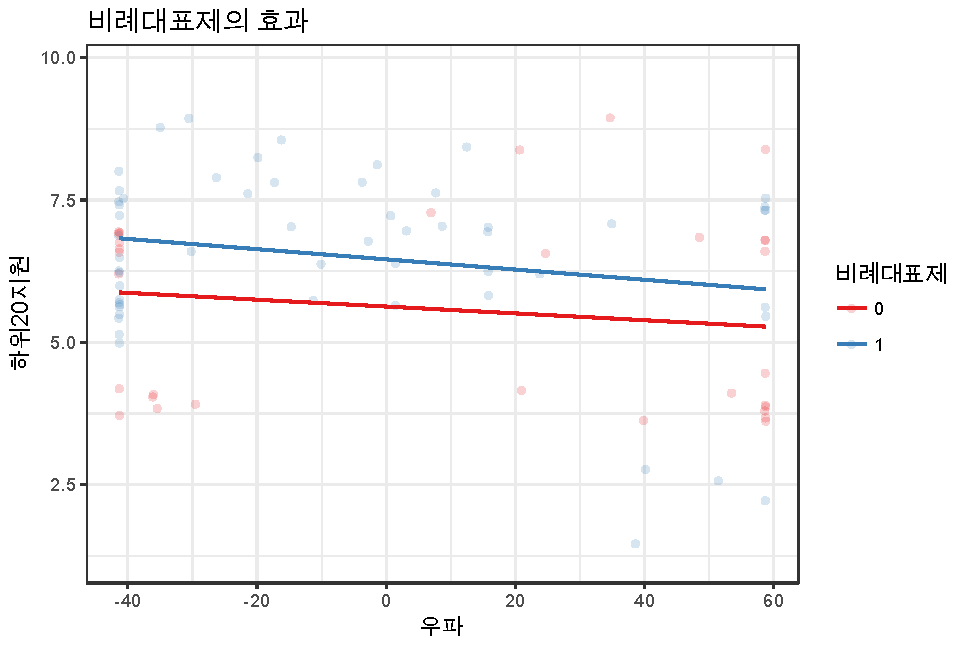
\includegraphics[width=0.9\textwidth]{pr_right.pdf}\\
        \caption{우파정당}
\end{figure}

바르텔즈(2017)는 여론동학(Dynamics)의 주장이 경험적으로 근거가 빈약하다고 반응한다. 여론조사에서 복지에 대한 수요가 공급을 압도함에도 여론과는 반대로 소위 '복지적자'가 발행하는 까닭은 정부가 담당해야 할 과도한 재정적 부담때문이다. Brooks \& Manza가 사회정책에 대한 선호로 사용한 "대중의 정책선호(mass policy preferences)\footnote{이들은 설문 다음의 두 가지를 이용하였다: 1) “On the whole, do you think it should or should not be the government’s responsibility to provide a job for everyone who wants one?” 2) “On the whole, do you think it should or should not be the government’s responsibility to reduce income differences between the rich and the poor?”.}를 기준하면 수요는 66.2\%인데 비해 비선호는 17.1\%로 49.6\%의 거대한 격차가 있다. \footnote{자료는 ISSP Social Inequality Module I-IV, 1987-2009를 이용했다. 바르텔즈(2017, p. 19)는 '복지국가지지(welfare state support)'라는 이름으로 이를  제시했다.}  바르폐즈는 시민의 선호가 정책으로 반영되지 않음을 지적하면서 모든 시민의 이해가 동일하게 반영되지 않는다고 주장한다. 빈곤층이 부유층과 다른 선호를 가지며 따라서 정책도 다른 종류를 원한다. 계급편견(class bias)이 작동하기 때문에 다수의 선호는 정책으로 나타날 수 없다는 것이다. 

바르텔즈는 연금, 의료, 교육 및 실업 등 주요 사회보험에 대한 선호를 평균하여 "사회지출선호(social spending preferences)"를 만들어\footnote{4개 분야 지출에 대한 선호 1-5를 0-100 구간으로 재구획하여 평균했다} 이를 기반으로 평균값이 50을 초과하면 초과수요라 개념화하고 복지적자(welfare deficits)를 제안했다.  이는 브룩스와 맨자가 만든 "포괄적 복지(mass social policy preferences)"
\end{document}